% Copyright (C) 2007 Technical University of Liberec.  All rights reserved.
%
% Please make a following reference to Flow123d on your project site if you use the program for any purpose,
% especially for academic research:
% Flow123d, Research Centre: Advanced Remedial Technologies, Technical University of Liberec, Czech Republic
%
% This program is free software; you can redistribute it and/or modify it under the terms
% of the GNU General Public License version 3 as published by the Free Software Foundation.
%
% This program is distributed in the hope that it will be useful, but WITHOUT ANY WARRANTY;
% without even the implied warranty of MERCHANTABILITY or FITNESS FOR A PARTICULAR PURPOSE.
% See the GNU General Public License for more details.
%
% You should have received a copy of the GNU General Public License along with this program; if not,
% write to the Free Software Foundation, Inc., 59 Temple Place - Suite 330, Boston, MA 021110-1307, USA.
%
%%%%%%%%%%%%%%%%%%%%%%%%%%%%%%%%%%%%%%%%%%%%%%%%%%%%%%%%%%%%%%%%%%
%
% use PDFLatex to compile this
%

\documentclass{llncs}

% our own flow_doc.sty
%\usepackage{flow_doc}

%\usepackage{rotating}
%\usepackage{pdflscape}

\usepackage{amssymb, amsmath}


\usepackage{array}
\usepackage{longtable}
\usepackage[usenames,dvipsnames]{color}   %colors
%\usepackage{colortbl}   %colorful tables
\usepackage{tabularx}
\usepackage{graphicx} %[dvips]
% it is note used \usepackage{cooltooltips}

%these two can be found in caption package
%\usepackage{caption}
%\usepackage{subcaption}

\usepackage[numbers]{natbib}

%\usepackage{fancyvrb}   % extended verbatim environments (for examples of IO files)

%\usepackage{multicol}
\usepackage{etoolbox}


%%%%%%%%%%%%%%%%%%%%%%%%%%%%%%%%%%%%%%%%%%%%%%%%%%%%%%%%%%%%%%%%%%%%%%%%%%%%
% macro for units 
\def\UNIT#1#2{\ifstrempty{#2}{}{%
\ifstrequal{#2}{1}{\mathrm{#1}}{\mathrm{#1}^{#2}}%
}}
\def\units#1#2#3{\ifstrempty{#1#2#3}{$[-]$}{$[ \UNIT{kg}{#1}\UNIT{m}{#2}\UNIT{s}{#3} ]$}}       %with brackets
\def\unitss#1#2#3{\ifstrempty{#1#2#3}{$-$}{$ \UNIT{kg}{#1}\UNIT{m}{#2}\UNIT{s}{#3} $}}  %without brackets


\newcommand{\vari}[1]{{\it #1}}
\newcommand{\ditem}[2]{\item[\vari{#1} {\tt #2}]}
\newenvironment{fileformat}{\tt\begin{flushleft}}{\end{flushleft}}

%%%%%%%%%%%%%%%%%%%% specific math macros
\def\prtl{\partial}
\def\vc#1{\mathbf{\boldsymbol{#1}}}     % vector
\def\tn#1{{\mathbb{#1}}}    % tensor
\def\abs#1{\lvert#1\rvert}
\def\Abs#1{\bigl\lvert#1\bigr\rvert}
\def\div{\operatorname{div}}
\def\ep{\varepsilon}
\def\Lapl{\Delta}
\def\grad{\nabla}
\def\Real{{\mathbf R}}
\def\d {\,{\rm d}}
\def\Natural{\mathbf N}
\def\norm#1{\|#1\|}
\def\yy{{\vc y}}
\def\ul{\underline}
\def\ol{\overline}

\renewcommand{\note}[2]{{\color{blue} \textbf{ #1:} \textit{#2}}}
%% ini_table members
%%%%%%%%%%%%%%%%%%%% specific math macros


%%%%%%%%%%%%%%%%%%%%%%%%%%%%%%%%%%%%%%%%%%%%%%%%%%%%%%%%%%%%%%%%%%%%%%%%%%%%%%%%%%%%%%%%%%%%% BEGIN DOCUMENT
%% set specific page layout
%\addtolength{\textwidth}{2cm}
%\addtolength{\hoffset}{-1.5cm}
%\addtolength{\textheight}{4cm}
%\addtolength{\voffset}{-2.5cm}
\begin{document}

\title{}
\author{Jan B\v rezina \and Jan Stebel}
\institute{Technical University of Liberec, Studentsk\'a 1402/2, 46117 Liberec, Czech Republic\\\email{\{jan.brezina,jan.stebel\}@tul.cz}}

\maketitle

\begin{abstract}
\end{abstract}

\section{Introduction}


Deep subsurface deposits in plutonic rock represent one of possible solution for final storage of nuclear waste. The primary reason is 
small hydraulic permeability of the bulk rock and thus slow migration of a possible leakage due to ground water flow.  On the other hand, 
granitoid formations contain fractures that may form a network of preferential paths with low volumetric water flow rate but with 
high velocity. The preferential paths pose a risk of fast transport of small amount of contaminant but in potentially dangerous concentrations.
The large scale effect of the small scale fractures is challenging for numerical simulations since direct discretization requires highly refined
computational mesh. One possible solution is to model fractures as lower dimensional objects and introduce their coupling with surrounding continuum.
A model for saturated flow in the system matrix-fracture was formally derived in \cite{martin_modeling_2005} by integrating the equations across the fracture.
It was justified by an error estimate $O(\max\{h,\delta\})$, $h$ being the mesh size and $\delta$ the fracture width, which holds inside the fracture for the solution of a particular mixed finite element approximation.
The approach was then generalized by others e.g. to the case of curved fractures with variable width \cite{angot_asymptotic_2009}, non-matching grids \cite{frih_modeling_2012} or to other equations or systems \cite{lesinigo_multiscale_2011,fumagalli_reduced_2013,ganis_modeling_2014}.
While most papers aim at the analysis or numerical solution of the continuum-fracture model, the precise statement declaring the relation of the original and reduced problem on the continuous level is, to our knowledge, missing.

In this paper we shall study the Darcy flow model, namely
\begin{equation}
\label{eq:darcy_flow}
\left.
\begin{aligned}
    \div \vc q &= f &&\mbox{ in }\Omega, \\
    \vc q &= -\tn K \grad p &&\mbox{ in }\Omega,\\
    p &= p_0 &&\mbox{ on }\partial\Omega,
\end{aligned}
\right\}
\end{equation}
where $\vc q$ is the Darcy flux, $f$ is the source density, $\tn K$ is the hydraulic conductivity tensor, $p$ is the piezometric head and $p_0$ is 
the piezometric head on the boundary.
In what follows, $\Omega \subset \Real^d$, $d=2,3$ will be a bounded domain with Lipschitz boundary (see Figure \ref{fig:omegas}, left), divided into the fracture
\[ \Omega_f:=\Omega\cap \big((-\delta/2,\delta/2)\times\Real^{d-1}\big) \]
with thickness $\delta>0$, and the surrounding set $\Omega_m:=\Omega\setminus\overline\Omega_f$, called the matrix.
The fracture interacts with the matrix on the interfaces 
\[ \gamma_1:=\Omega\cap\big( \{-\delta/2\}\times \Real^{d-1}\big) \mbox{ and }\gamma_2:=\Omega\cap\big( \{ \delta/2\}\times \Real^{d-1}\big). \]
Normal vectors on these interfaces are denoted $\vc n_i$, $i=1,2$ with the orientation out of $\Omega_m$.
Further, we introduce the reduced geometry (see Figure \ref{fig:omegas}, right)
where the fracture is represented by the interface $\gamma:=\Omega\cap\big(\{0\}\times\Real^{d-1}\big)$ in its center.
For any point $\vc x\in\Real^d$ we shall write $\vc x=(x,\yy)^\top$, $\yy\in\Real^{d-1}$.
For functions defined in $\Omega_f$ we define the tangent gradient along the fracture
\[ \nabla_\yy v:=(0,\partial_{y_1} v,\ldots,\partial_{y_{d-1}} v)^\top, \]
and the average of $v$ across the fracture:
\[ \bar v:=\frac1\delta\int_{-\delta/2}^{\delta/2} v(x,\cdot)\,dx. \]
\begin{figure}[h]
\centering
\includegraphics[width=12cm]{figures/full_model_domain}
\label{fig:omegas}
\caption{The domain of the full model (left) and the reduced geometry (right).}
\end{figure}

We shall study the relation of \eqref{eq:darcy_flow} to the so-called \emph{continuum-fracture model} on the reduced geometry:
\begin{equation}
\label{eq:asymptotic_darcy}
\left.
\begin{aligned}
-\div(\tn K\nabla p_m) &= f &&\mbox{ in }\Omega_m,\\
p_m &= p_0 &&\mbox{ on }\partial\Omega\cap\partial\Omega_m,\\
-\tn K\nabla p_m\cdot\vc n_i &= q_i(p_m,p_f) &&\mbox{ on }\gamma_i,~i=1,2,\\
-\div(\delta\tn K\nabla_\yy p_f) &= \delta\bar f + \sum_{i=1}^2 q_i(p_m,p_f) &&\mbox{ in }\gamma,\\
p_f &= p_0 &&\mbox{ on }\overline\gamma\cap\partial\Omega.
\end{aligned}
\right\}
\end{equation}
The fluxes $q_1$, $q_2$ between the fracture and the matrix are defined as follows:
\[ q_i(v,w):=\frac{2\tn K_{|\gamma}\vc n_i\cdot\vc n_i}\delta (v_{|\gamma_i}-w_{|\gamma}), ~v\in H^1(\Omega_m),~w\in L^2(\gamma), ~i=1,2. \]
Our goal is to justify \eqref{eq:asymptotic_darcy} as an approximation of \eqref{eq:darcy_flow} in the case when $\delta$ is small.
In particular, we shall prove that
\[ \bar u - u_f \approx \delta\quad\mbox{and}\quad u_{|\Omega_m}-u_m \approx \delta^{3/2} \]
in a suitable sense.


The organization of the paper is as follows.
In the next section we formulate and prove the main theoretical result on the error analysis.
Then, in section \ref{sc:numerics} we show numerical results which confirm the error estimates.









\section{Asymptotic properties of continuum-fracture model}


In what follows we assume that $\tn K$ is uniformly positive definite, bounded in $\Omega$ and has the following form:
\[ \tn K = \begin{cases}\tn K_m & \mbox{ in }\Omega_m,\\ \tn K_f = \begin{pmatrix}k_x & 0\\0&\tn K_\yy\end{pmatrix} & \mbox{ in }\Omega_f,\end{cases} \]
where $\tn K_f(x,\yy)=\tn K_f(\yy)$.
Further we consider right hand side $f\in L^2(\Omega)$.
As the problem is linear, we can set $p_0\equiv 0$ without loss of generality.


\subsection{Weak formulation}

The ongoing analysis will be done in the framework of weak solutions.
We say that $p\in H^1_0(\Omega)$ is the weak solution of \eqref{eq:darcy_flow} if for every $v\in H^1_0(\Omega)$:
\begin{equation}
\label{eq:weak_darcy}
\int_\Omega \tn K\nabla p\cdot\nabla v = \int_\Omega f v.
\end{equation}
Introducing the space
\[ H^1_{bc}(\Omega_m) := \{v\in H^1(\Omega_m);~v_{|\partial\Omega_m\cap\partial\Omega}=0\}, \]
we analogously define the weak solution of \eqref{eq:asymptotic_darcy} as the couple $(p_m,p_f)\in H^1_{bc}(\Omega_m)\times H^1_0(\gamma)$ that satisfies
% \begin{subequations}
% \label{eq:weak_asym}
% \begin{equation}
% \int_{\Omega_m}\tn K_m\nabla p_m\cdot\nabla v_m + \sum_{i=1}^2\int_\gamma q_i(p_m,p_f)v_{m|\gamma_i} = \int_{\Omega_m} f v_m,
% \end{equation}
% \begin{equation}
% \delta\int_{\gamma}\tn K_\yy\nabla_\yy p_f\cdot\nabla_\yy v_f = \delta\int_\gamma\bar f v_f + \sum_{i=1}^2\int_\gamma q_i(p_m,p_f)v_f
% \end{equation}
\begin{multline}
\label{eq:weak_darcy_short}
\int_{\Omega_m}\tn K_m\nabla p_m\cdot\nabla v_m
+\delta\int_{\gamma}\tn K_\yy\nabla_\yy p_f\cdot\nabla_\yy v_f\\
+ \sum_{i=1}^2\int_{\gamma_i} q_i(p_m,p_f)(v_{m|\gamma_i} - v_f)
 = \int_{\Omega_m} f v_m + \delta\int_\gamma\bar f v_f
\end{multline}
for all $(v_m,v_f)\in H^1_{bc}(\Omega_m)\times H^1_0(\gamma)$.
% \end{subequations}
% We shall also use a compact form of \eqref{eq:weak_asym}, namely

Let us remark that under the above assumptions on $\tn K$ and $f$, problems \eqref{eq:weak_darcy} and \eqref{eq:weak_darcy_short} have unique solutions.



\subsection{Error analysis of asymptotic model}
\label{sc:error_estimate}

% (note: $p\in H^1(\Omega_f)\Rightarrow\bar p\in H^1(\gamma)$)


Let $\sigma(\tn A)$ denote the spectrum of a matrix $\tn A$.
We make the following notation:
\[ \underline K_m := \inf_{\vc x\in\Omega_m}\sigma(\tn K_m(\vc x)), \quad \underline K_\yy := \inf_{\vc x\in\Omega_f}\sigma(\tn K_\yy(\vc x)), \]
\[ \underline k_x := \inf_{\yy\in\gamma}k_x(\yy), \quad \overline k_x:=\sup_{\yy\in\gamma}k_n(\yy). \]
The main result of this section is the following error estimate.
\begin{theorem}
\label{th:error_estimate}
Let $\delta>0$, and assume in addition that the unique solution to \eqref{eq:weak_darcy} satisfies
\[ \partial_x^2 p\in L^q(\Omega_f), ~q\in[2,\infty]. \]
Then there is a constant $C:=C(\Omega,\gamma)>0$ independent of $\delta$, $\tn K$ and $f$ such that
\begin{subequations}
\label{eq:error_estimates_delta}
\begin{align}
&\norm{\nabla_\yy(\bar p - p_f)}_{2,\gamma} \le C\sqrt{\frac{\overline k_x}{\underline K_\yy}}\norm{\partial_x^2 p}_{q,\Omega_f}\delta^{1-\frac1q},\\
&\norm{\nabla(p-p_m)}_{2,\Omega_m} \le C\sqrt{\frac{\overline k_x}{\underline K_m}}\norm{\partial_x^2 p}_{q,\Omega_f}\delta^{\frac32-\frac1q},\\
&\sum_{i=1}^2\norm{\bar p-p_{|\gamma_i}+p_{m|\gamma_i}-p_f}_{2,\gamma} \le C\sqrt{\frac{\overline k_x}{\underline k_x}}\norm{\partial_x^2 p}_{q,\Omega_f}\delta^{2-\frac1q},
\end{align}
\end{subequations}
where $(p_m,p_f)$ is the solution of \eqref{eq:weak_darcy_short}.
\end{theorem}


\begin{proof}
For any $\ep\in(0,\delta/2)$ we define the sets
\begin{align*}
\Omega_{f\ep} &:= \{(x,\vc y)\in\Omega;~-\delta/2+\ep<x<\delta/2-\ep\},\\
\Omega_{f\ep}^- &:= \{(x,\vc y)\in\Omega_f;~x<-\delta/2+\ep\},\\
\Omega_{f\ep}^+ &:= \{(x,\vc y)\in\Omega_f;~x>\delta/2-\ep\}
\end{align*}
and an auxiliary operator $\Pi_\ep:L^2(\Omega_m)\times L^2(\gamma)\to L^2(\Omega)$:
\[ \Pi_\ep(v_m,v_\gamma)(x,\vc y) :=
\begin{cases}
v_m(x,\vc y) & \mbox{ in }\Omega_m,\\
v_\gamma(0,\vc y) & \mbox{ in }\Omega_{f\ep},\\
\frac1\ep(x+\frac\delta2)v_\gamma(0,\vc y) - \frac1\ep(x+\frac\delta2-\ep)v_m(-\frac\delta2,\vc y) & \mbox{ in }\Omega_{f\ep}^-,\\
-\frac1\ep(x-\frac\delta2)v_\gamma(0,\vc y) + \frac1\ep(x-\frac\delta2+\ep)v_m(\frac\delta2,\vc y) & \mbox{ in }\Omega_{f\ep}^+.
\end{cases}
\]
Note that $\Pi_\ep$ maps $H^1_{bc}(\Omega_m)\times H^1_0(\gamma)$ into $H^1_0(\Omega)$.
We use $v_\ep:=\Pi_\ep(v_m,v_f)$, $v_m\in H^1_{bc}(\Omega_m)$, $v_f\in H^1_0(\gamma)$ as a test function in \eqref{eq:weak_darcy}:
% $v_\ep:=\Pi_\ep(p-p_m,\bar p-p_f)$, where $p$, $p_m$ and $p_f$ satisfy \eqref{eq:weak_darcy} and \eqref{eq:weak_darcy_short}, respectively:
% \begin{multline}
% \label{eq:global_vk}
% \int_{\Omega_m}\tn K_m\nabla p\cdot\nabla(p-p_m)
% +\int_{\Omega_{f\ep}}\tn K_t\nabla_\yy p\cdot\nabla_\yy(\bar p-p_f)
% +\int_{\Omega_f\setminus\Omega_{f\ep}} k_n\partial_x p \partial_x v_\ep\\
% + \int_{\Omega_f\setminus\Omega_{f\ep}} \tn K_t\nabla_\yy p \cdot \nabla_\yy\Pi_\ep(p-p_m,\bar p-p_f)
% = \int_{\Omega_m} f_p (p-p_m)\\
% + \int_{\Omega_{f\ep}} f_p (\bar p-p_f)
% + \int_{\Omega_f\setminus\Omega_{f\ep}} f_p v_\ep.
% \end{multline}
\begin{multline}
\label{eq:global_veps}
\int_{\Omega_m}\tn K_m\nabla p\cdot\nabla v_m
+\int_{\Omega_{f\ep}}\tn K_\yy\nabla_\yy p\cdot\nabla_\yy v_f
+\int_{\Omega_f\setminus\Omega_{f\ep}} k_x\partial_x p \partial_x v_\ep\\
+ \int_{\Omega_f\setminus\Omega_{f\ep}} \tn K_\yy\nabla_\yy p \cdot \nabla_\yy v_\ep
= \int_{\Omega_m} f v_m
+ \int_{\Omega_{f\ep}} f v_f
+ \int_{\Omega_f\setminus\Omega_{f\ep}} f v_\ep.
\end{multline}
Next we shall perform the limit $\ep\to 0+$.
Due to continuity of integral we have:
\begin{align}
&\int_{\Omega_{f\ep}}\tn K_\yy\nabla_\yy p\cdot\nabla_\yy v_f \to \int_{\Omega_f}\tn K_\yy\nabla_\yy p\cdot\nabla_\yy v_f = \delta\int_\gamma\tn K_\yy\nabla_\yy\bar p\cdot\nabla_\yy v_f,\\
&\int_{\Omega_f\setminus\Omega_{f\ep}} \tn K_\yy\nabla_\yy p \cdot \nabla_\yy v_\ep \to 0, \\
&\int_{\Omega_{f\ep}} f v_f \to \int_{\Omega_f} f v_f = \delta\int_{\gamma} \bar f v_f, \\
&\int_{\Omega_f\setminus\Omega_{f\ep}} f v_\ep \to 0,~\ep\to 0+.
\end{align}
The remaining term can be rewritten as follows:
\begin{multline}
\int_{\Omega_f\setminus\Omega_{f\ep}} k_x\partial_x p \partial_x v_\ep
= \frac1\ep\int_{\Omega_{f\ep}^-} k_x\partial_x p (v_f-v_{m|\gamma_1})
- \frac1\ep\int_{\Omega_{f\ep}^+} k_x\partial_x p (v_f - v_{m|\gamma_2})\\
\to \sum_{i=1}^2(-1)^{1+i}\int_\gamma k_x \partial_x p_{|\gamma_i} (v_f - v_{m|\gamma_i}),~\ep\to 0+.
\end{multline}
Let $\vc y\in\Real^{d-1}$ be fixed and define
\[ P(x):=\frac1\delta\int_{-\delta/2}^{x}p(t,\vc y)~dt. \]
Using the Taylor expansion 
\begin{multline}
P(x) = P(-\delta/2) + (x+\frac\delta2)P'(-\delta/2) + \frac{(x+\frac\delta2)^2}{2}P''(-\delta/2)\\
+ \frac{(x+\frac\delta2)^2}2\int_{-\delta/2}^{\xi(x,\vc y)}P'''(t)~dt,~\xi(x,\vc y)\in(-\delta/2,x),
\end{multline}
we can show that
\[ \bar p(\vc y) = P(\delta/2) = p(-\delta/2,\vc y) + \frac\delta2\partial_x p(-\delta/2,\vc y) + \frac\delta2\int_{-\delta/2}^{\xi(\delta/2,\vc y)}\partial_x^2 p(t,\vc y)~dt. \]
By a similar argument we obtain:
\[ \bar p(\vc y) = p(\delta/2,\vc y) - \frac\delta2\partial_x p(-\delta/2,\vc y) + \frac\delta2\int_{\eta(-\delta/2,\vc y)}^{\delta/2}\partial_x^2 p(t,\vc y)~dt,~\eta(x,\vc y)\in(x,\delta/2). \]
From this we can deduce that
\begin{equation}
\label{eq:taylor_for_du}
\partial_x p_{|\gamma_i} = (-1)^{1+i}\left(\frac2\delta(\bar p - p_{|\gamma_i}) - \delta g_i\right),~i=1,2,
\end{equation}
where
\begin{equation}
\label{eq:estimate_gi}
|g_i(\vc y)| \le \frac1\delta\int_{-\delta/2}^{\delta/2} |\partial_x^2 p(\cdot,\vc y)|.
\end{equation}
Summing up, \eqref{eq:global_veps}--\eqref{eq:taylor_for_du} yields:
\begin{multline}
\label{eq:sum_global_vk_limit}
\int_{\Omega_m}\tn K_m\nabla p\cdot\nabla v_m
+\delta\int_\gamma\tn K_\yy\nabla_\yy\bar p\cdot\nabla_\yy v_f
+ \sum_{i=1}^2\int_{\gamma_i} q_i(p,\bar p) (v_{m|\gamma_i} - v_f)\\
= \int_{\Omega_m} f v_m
+ \delta\int_{\gamma} \bar f v_f
+ \delta\sum_{i=1}^2\int_\gamma k_x g_i\, (v_{m|\gamma_i} - v_f).
\end{multline}
% \begin{multline}
% \label{eq:sum_global_vk_limit}
% \int_{\Omega_m}\tn K_m\nabla p\cdot\nabla(p-p_m)
% +\delta\int_\gamma\tn K_t\nabla_\yy\bar p\cdot\nabla_\yy(\bar p-p_f)\\
% + \sum_{i=1}^2\int_\gamma q(\bar p,p_{|\gamma_i}) (\bar p - p_{|\gamma_i} + p_{m|\gamma_i} - p_f)\\
% = \int_{\Omega_m} f_p (p-p_m)
% + \delta\int_{\gamma} \bar f_p (\bar p-p_f)
% + \delta\sum_{i=1}^2\int_\gamma k_n g_i\, (\bar p - p_{|\gamma_i} + p_{m|\gamma_i} - p_f).
% \end{multline}

Now we use $v_m:=p-p_m$, $v_f:=\bar p-p_f$ as test functions in \eqref{eq:sum_global_vk_limit} and \eqref{eq:weak_darcy_short}, and subtract the resulting identities.
We obtain:
\begin{multline}
\label{eq:difference}
\int_{\Omega_m}\tn K_m\nabla(p-p_m)\cdot\nabla(p-p_m)
+ \delta\int_\gamma\tn K_\yy\nabla_\yy(\bar p-p_f)\cdot\nabla_\yy(\bar p-p_f)\\
+ \sum_{i=1}^2\int_{\gamma} \frac{2k_x}\delta |p_{|\gamma_i} - p_{m|\gamma_i} - \bar p + p_f|^2
= \delta\sum_{i=1}^2\int_\gamma k_x g_i\, (p_{|\gamma_i}-p_{m|\gamma_i} - \bar p + p_f).
\end{multline}
Using H\"older's and Young's inequality we can estimate the right hand side of \eqref{eq:difference}:
\begin{multline}
\label{eq:estimate_rhs}
\delta\sum_{i=1}^2\int_\gamma k_x g_i\, (p_{|\gamma_i}-p_{m|\gamma_i} - \bar p + p_f)\\
\le \frac{\delta^{\frac32}}{\sqrt2}\sum_{i=1}^2\int_\gamma \sqrt{k_x}|g_i|\sqrt{\frac{2k_x}\delta}|p_{|\gamma_i}-p_{m|\gamma_i} - \bar p + p_f|\\
\le \frac{\delta^3}4\overline k_x\sum_{i=1}^2\norm{g_i}_{2,\gamma}^2 + \frac12\sum_{i=1}^2\int_\gamma \frac{2k_x}\delta |p_{|\gamma_i}-p_{m|\gamma_i} - \bar p + p_f|^2.
\end{multline}
From \eqref{eq:estimate_gi} and H\"older's inequality it follows that
\begin{equation}
\label{eq:estimate_gi_l2}
\norm{g_i}_{2,\gamma}^2 \le \delta^{-\frac2q}|\gamma|^{\frac{q-2}q}\norm{\prtl_x^2 p}_{q,\Omega_f}^2.
\end{equation}
Finally, \eqref{eq:difference}, \eqref{eq:estimate_rhs}, \eqref{eq:estimate_gi_l2} and the uniform positive definiteness of $\tn K$ yields:
\begin{multline}
\underline K_m\norm{\nabla (p-p_m)}_{2,\Omega_m}^2
+\delta\underline K_\yy\norm{\nabla_\yy(\bar p-p_f)}_{2,\gamma}^2\\
+ \frac1\delta\underline k_x\sum_{i=1}^2\norm{\bar p - p_{|\gamma_i} + p_{m|\gamma_i} - p_f}_{2,\gamma}^2
\le \frac{\overline k_x}2|\gamma|^{\frac{q-2}q}\norm{\partial_x^2 p}_{q,\Omega_f}^2\delta^{3-\frac2q},
\end{multline}
from which the estimates \eqref{eq:error_estimates_delta} follow.
\end{proof}




\section{Numerical experiments}
\label{sc:numerics}

\note{JS}{
OUR STRATEGY - compare two models using 2nd order approximation in space + meshes refined proportionally to cross section.
\\
DESCRIBE FLOW123D - mixed-hybrid method for Darcy flow, DG for transport, input/output interface
\\
TEST PROBLEMS - analytical solutions, tests from JMR paper, comments to the results
}

In this section we present computational results that demonstrate the relevance of the continuum-fracture model in the discrete setting, in particular we study the dependence of the error between the full and the reduced model on the fracture cross section.
For this reason we choose numerical methods with 2nd order accuracy in space with respect to the $L^2$ norm and a sequence of computational meshes with the norm $h\approx\delta$. Consequently we are able to observe the order $O(\delta)$ and $O(\delta^{3/2})$, respectively, of the respective error norms.

In all computations we shall use the domain $\Omega:=(-1,1)\times(0,1)$ and the fracture $\Omega_f^\delta:=(-\delta/2,\delta/2)\times(0,1)$.

For the Darcy flow we measure the $L^2$ error in the piezometric head in $\Omega_m^\delta:=\Omega\setminus\Omega_f^\delta$ and $\gamma$:
\[ e_m^\delta := \norm{p^\delta - p_m^\delta}_{2,\Omega_m^\delta},\quad e_f^\delta := \norm{p^\delta - p_f^\delta}_{2,\gamma}. \]


\subsection{Test case 1 - harmonic pressure}

Data: $\tn K=\tn I$, $f_p=0$, left/right - nonhomogeneous Dirichlet b.c., top/bottom - nonhomogeneous Neumann b.c.
Exact solution:
\[ p(x,y) = e^x\sin y \]
According to Theorem \ref{th:error_estimate}, the errors should behave as follows: $e_m^\delta\approx\delta^{3/2}$, $e_f^\delta\approx\delta$.

\begin{tabular}{|l|ll|ll|}
\hline
$\delta$ & $(e_m^\delta)^2$ & EOC (matrix) & $(e_f^\delta)^2$ & EOC (fracture)\\
\hline
4.00e-01 & 2.4899e-03 &            & 1.9525e-03 & \\
2.00e-01 & 2.5948e-04 & 1.6312e+00 & 2.7821e-04 & 1.4055e+00\\
1.00e-01 & 3.1960e-05 & 1.5106e+00 & 5.2709e-05 & 1.2000e+00\\
5.00e-02 & 3.5416e-06 & 1.5869e+00 & 1.1414e-05 & 1.1036e+00\\
2.50e-02 & 4.3285e-07 & 1.5162e+00 & 2.6676e-06 & 1.0486e+00\\
1.25e-02 & 5.3499e-08 & 1.5081e+00 & 6.4513e-07 & 1.0239e+00\\
6.25e-03 & 6.6789e-09 & 1.5009e+00 & 1.5865e-07 & 1.0119e+00\\
\hline
Expected & & 1.5 & & 1\\
\hline
\end{tabular}

% % The following results were wrong, in fact we get the same orders as above (1.5, 1)
% Next, we scale the conductivity tensor $\tn K_f:=\frac1\delta\tn I$ and use the same boundary conditions. The exact solution remains the same.
% The expected order is now $e_m^\delta\approx\delta$, $e_f^\delta\approx\delta$.
% 
% \begin{tabular}{|l|ll|ll|}
% \hline
% $\delta$ & $(e_m^\delta)^2$ & EOC (matrix) & $(e_f^\delta)^2$ & EOC (fracture)\\
% \hline
% 4.00e-01 & 6.8043e-03 &            & 1.6771e-02 & \\
% 2.00e-01 & 1.6164e-03 & 1.0368e+00 & 3.9297e-03 & 1.0467e+00\\
% 1.00e-01 & 4.0703e-04 & 9.9478e-01 & 9.6050e-04 & 1.0163e+00\\
% 5.00e-02 & 1.0201e-04 & 9.9824e-01 & 2.3074e-04 & 1.0287e+00\\
% 2.50e-02 & 2.5552e-05 & 9.9859e-01 & 5.7078e-05 & 1.0076e+00\\
% 1.25e-02 & 6.3936e-06 & 9.9936e-01 & 1.4200e-05 & 1.0035e+00\\
% 6.25e-03 & 1.5991e-06 & 9.9969e-01 & 3.5465e-06 & 1.0007e+00\\
% \hline
% Expected & & 1 & & 1\\
% \hline
% \end{tabular}



\subsection{Test case 2 - nonzero source}

Data: $\tn K=\tn I$, $f_p=2y-1$, left/right - nonhomogeneous Dirichlet, top/bottom - homogeneous Neumann b.c.
Exact solution:
\[ p(x,y) = -\frac{x}2 - \frac{y^3}3 + \frac{y^2}2 \]
Expected order: $e_m^\delta\approx\delta^{3/2}$, $e_f^\delta\approx\delta$.

\begin{tabular}{|l|ll|ll|}
\hline
$\delta$ & $(e_m^\delta)^2$ & EOC (matrix) & $(e_f^\delta)^2$ & EOC (fracture)\\
\hline
4.00e-01 & 2.7352e-03 &            & 3.2885e-05 &           \\
2.00e-01 & 3.4103e-04 & 1.5018e+00 & 7.8094e-06 & 1.0371e+00\\
1.00e-01 & 4.5694e-05 & 1.4499e+00 & 1.8929e-06 & 1.0223e+00\\
5.00e-02 & 5.3165e-06 & 1.5517e+00 & 4.6537e-07 & 1.0121e+00\\
2.50e-02 & 6.6431e-07 & 1.5003e+00 & 1.1540e-07 & 1.0059e+00\\
1.25e-02 & 8.3023e-08 & 1.5001e+00 & 2.8731e-08 & 1.0030e+00\\
6.25e-03 & 1.0419e-08 & 1.4971e+00 & 7.1679e-09 & 1.0015e+00\\
\hline
Expected & & 1.5 & & 1\\
\hline
\end{tabular}

Transport: zero initial condition, $\theta=0.1$, right: Dirichlet b.c. $1$, time interval $(0,0.45)$
Zero diffusion:

\begin{tabular}{|l|ll|ll|}
\hline
$\delta$ & $(e_m^\delta)^2*0.45$ & EOC (matrix) & $(e_f^\delta)^2*0.45$ & EOC (fracture)\\
\hline
4.00e-01 & 3.3746e-01 &            & 2.3598e-03 &           \\ 
2.00e-01 & 1.9794e-01 & 5.0865e-01 & 1.8645e-02 & 6.6722e-01\\  
1.00e-01 & 8.3739e-02 & 7.7955e-01 & 1.0253e-02 & 5.8354e-01\\
5.00e-02 & 2.2839e-02 & 1.0578e+00 & 2.9655e-03 & 8.4844e-01\\
2.50e-02 & 3.6513e-03 & 1.3804e+00 & 7.3713e-04 & 9.6713e-01\\
1.25e-02 & 3.9963e-04 & 1.6179e+00 & 1.7860e-04 & 1.0001e+00\\
6.25e-03 & 3.6526e-05 & 1.7325e+00 & 4.3463e-05 & 1.0062e+00\\
\hline
Expected & & ? & & ?\\
\hline
\end{tabular}

Diffusion $\tn D=0.1\tn I$:

\begin{tabular}{|l|ll|ll|}
\hline
$\delta$ & $(e_m^\delta)^2*0.45$ & EOC (matrix) & $(e_f^\delta)^2*0.45$ & EOC (fracture)\\
\hline
4.00e-01 & 7.1668e-02 &            & 2.8439e-02 &            \\
2.00e-01 & 2.4313e-02 & 1.1239e+00 & 1.9724e-02 & 7.1121e-01 \\
1.00e-01 & 2.5986e-03 & 1.6569e+00 & 3.7972e-03 & 1.1298e+00 \\
5.00e-02 & 1.6395e-04 & 2.0134e+00 & 6.5148e-04 & 1.2219e+00 \\
2.50e-02 & 1.7331e-05 & 1.7132e+00 & 9.9551e-05 & 1.3395e+00 \\
1.25e-02 & 1.5975e-06 & 1.7456e+00 & 1.2088e-05 & 1.5115e+00 \\
6.25e-03 & 1.2553e-07 & 1.8268e+00 & 1.1732e-06 & 1.6769e+00 \\
\hline
Expected & & ? & & ?\\
\hline
\end{tabular}


%\section{Heat transfer}

Under the assumption of thermal equilibrium between the solid and liquid phase, the energy balance equation has the form\footnote{For lower dimensions this form can be derived as in Section \ref{sc:ad_on_fractures} using $w:=\delta\tilde s T$, $u:=T$, $\tn A:=\delta\lambda\tn I$, $\vc b:=\frac{\varrho_l c_l}{\tilde s}\vc w$.}
\[
    \partial_t\left(\delta \tilde s T \right) + \div(\varrho_l c_l T \vc q) - \div(\delta\Lambda\nabla T) = F^T + F^T_C.
\]
The principal unknown is the temperature $T$ [K].
Other quantities are:
\begin{itemize}
\item \hyperA{HeatTransfer-DG-Data::fluid-density}{$\varrho_l$}, \hyperA{HeatTransfer-DG-Data::solid-density}{$\varrho_s$} \units{1}{-3}{} is the density of the fluid and solid phase, respectively.
\item \hyperA{HeatTransfer-DG-Data::fluid-heat-capacity}{$c_l$}, \hyperA{HeatTransfer-DG-Data::solid-heat-capacity}{$c_s$} [J$\mathrm{kg}^{-1}\mathrm{K}^{-1}$] is the heat capacity of fluid and solid phase, respectively.
\item $\tilde s$ [J$\mathrm{m}^{-3}\mathrm{K}^{-1}$] is the volumetric heat capacity of the porous medium defined as
\[ \tilde s = \hyperA{HeatTransfer-DG-Data::porosity}{\th}\varrho_l c_l + (1-\th)\varrho_s c_s. \]
\item $\Lambda$ [W$\mathrm{m}^{-1}\mathrm{K}^{-1}$] is the thermal dispersion tensor:
\[ \Lambda = \Lambda^{cond} + \Lambda^{disp} \]
\[ \Lambda^{cond} = \left(\th \lambda_l^{cond} + (1-\th)\lambda_s^{cond}\right)\tn I, \]
\[ \Lambda^{disp} = \th \varrho_l c_l|\vc v|\left(\alpha_T\tn I + (\alpha_L-\alpha_T)\frac{\vc v\otimes\vc v}{|\vc v|^2}\right), \]
where \hyperA{HeatTransfer-DG-Data::fluid-heat-conductivity}{$\lambda_l^{cond}$}, \hyperA{HeatTransfer-DG-Data::solid-heat-conductivity}{$\lambda_s^{cond}$} [W$\mathrm{m}^{-1}\mathrm{K}^{-1}$] is the thermal conductivity of the fluid and solid phase, respectively, and \hyperA{HeatTransfer-DG-Data::disp-l}{$\alpha_L$}, \hyperA{HeatTransfer-DG-Data::disp-t}{$\alpha_T$} \units{}{1}{} is the longitudal and transverse dispersivity in the fluid.

\item $F^T$ [J$\mathrm{m}^{-d}\mathrm{s}^{-1}$] represents the thermal source:
\[ F^T = \delta \th F^T_l + \delta (1-\th) F^T_s, \]
\[ F^T_l = f_l^T + \varrho_l c_l \sigma^T_l(T-T_l), \]
\[ F^T_s = f_s^T + \varrho_s c_s \sigma^T_s(T-T_s), \]
where \hyperA{HeatTransfer-DG-Data::fluid-thermal-source}{$f_l^T$}, \hyperA{HeatTransfer-DG-Data::solid-thermal-source}{$f_s^T$} [W$\mathrm{m}^{-3}$] is the density of thermal sources in fluid and solid, respectively, \hyperA{HeatTransfer-DG-Data::fluid-ref-temperature}{$T_l$}, \hyperA{HeatTransfer-DG-Data::solid-ref-temperature}{$T_s$} [K] is a reference temperature and \hyperA{HeatTransfer-DG-Data::fluid-heat-exchange-rate}{$\sigma^T_l$}, \hyperA{HeatTransfer-DG-Data::solid-heat-exchange-rate}{$\sigma^T_s$} \units{}{}{-1} is the heat exchange rate.
\end{itemize}



\paragraph{Initial and boundary conditions.}
At time $t=0$ the temperature is determined by the initial condition
$$ T(0,\vc x) = \hyperA{HeatTransfer-DG-Data::init-temperature}{T_0}(\vc x). $$
Given the decomposition of $\partial\Omega_d$ into $\Gamma_I\cup\Gamma_D\cup\Gamma_N\cup\Gamma_R$ (see Section \ref{sc:transport_model}), we prescribe the following boundary conditions:
\begin{itemize}
\item Dirichlet:
\[ T = \hyperA{HeatTransfer-DG-Data::bc-temperature}{T_D} \mbox{ on }\Gamma_I^+\cup\Gamma_D, \]
\item Homogeneous Neumann:
\[ \left(\varrho_l c_l T \vc q - \delta\Lambda\nabla T\right)\cdot\vc n = 0 \mbox{ on }\Gamma_I^-, \]
\item Neumann:
\[ \left(\varrho_l c_l T \vc q - \delta\Lambda\nabla T\right)\cdot\vc n = \hyperA{HeatTransfer-DG-Data::bc-flux}{f_N} \mbox{ on }\Gamma_N, \]
\item Robin (Newton):
\[ \left(\varrho_l c_l T \vc q - \delta\Lambda\nabla T\right)\cdot\vc n = \hyperA{HeatTransfer-DG-Data::bc-robin-sigma}{\sigma_R}(T-\hyperA{HeatTransfer-DG-Data::bc-temperature}{T_D}) \mbox{ on }\Gamma_R. \]
\end{itemize}






\paragraph{Communication between dimensions.}
Denoting $T_{d+1}$, $T_d$ the temperature in $\Omega_{d+1}$ and $\Omega_d$, respectively, the communication on the interface between $\Omega_{d+1}$ and $\Omega_d$ is described by the quantity
\begin{equation}
  \label{e:inter_dim_flux_heat}
  q^T_{d+1,d} = \sigma^T_{d+1,d} \frac{\delta_{d+1}^2}{\delta_d}2\Lambda_d:\n\otimes\n ( T_{d+1} - T_d) + \begin{cases} \varrho_l c_l q^l_{d+1,d} T_{d+1} & \mbox{ if }q^l_{d+1,d}\ge 0,\\\varrho_l c_l q^l_{d+1,d} \frac{\tilde s_d}{\tilde s_{d+1}} T_d & \mbox{ if } q^l_{d+1,d}<0,\end{cases}
\end{equation}
where
\begin{itemize}
\item $q^T_{d+1,d}$ [W$\mathrm{m}^{-2}$] is the density of heat flux from $\Omega_{d+1}$ to $\Omega_d$,
\item \hyperA{HeatTransfer-DG-Data::fracture-sigma}{$\sigma^T_{d+1,d}$} \units{}{}{} is a transition parameter.
Its value determines the exchange of energy between dimensions due to temperature difference.
In general, it is recommended to leave the default value $\sigma^T=1$ or to set $\sigma^T=0$ (when exchange is due to water flux only).
\item $q^l_{d+1,d}=\vc q_{d+1}\cdot\vc n$ is the water flux from $\Omega_{d+1}$ to $\Omega_d$.
\end{itemize}
The communication between dimensions is incorporated as the total flux boundary condition for the problem on $\Omega_{d+1}$:
\begin{equation}
\label{e:heat_FC}
\left(\varrho_l c_l T \vc q - \delta\Lambda\nabla T\right)\cdot\vc n = q^T
\end{equation}
and a source term in $\Omega_d$:
\begin{equation}
F^T_{C3} = 0,\quad
F^T_{C2} = q^T_{32},\quad
F^T_{C1} = q^T_{21}.
\end{equation}




\paragraph{Energy balance.}
The heat equation satisfies the balance of energy in the following form:
$$ e(0) + \int_0^t s(\tau) \,d\tau - \int_0^t f(\tau) \,d\tau = e(t) $$
for any instant $t$ in the computational time interval.
Here
$$ e(t) := \sum_{d=1}^3\int_{\Omega^d}(\delta \tilde s T)(t,\vc x)\,d\vc x, $$
$$ s(t) := \sum_{d=1}^3\int_{\Omega^d}F_S^T(t,\vc x)\,d\vc x, $$
$$ f(t) := \sum_{d=1}^3\int_{\partial\Omega^d}\left(\varrho_l c_l T\vc q - \delta\Lambda\nabla T\right)(t,\vc x)\cdot\vc n \,d\vc x $$
is the energy [J], the volume source [J$\mathrm{s}^{-1}$] and the energy flux [J$\mathrm{s}^{-1}$] at time $t$, respectively.
The energy, flux and source on every geometrical region is calculated at each computational time step and the values together with the control sums are written to the file \texttt{mass\_balance.txt}.









\bibliographystyle{abbrvnat}
\bibliography{flow123d_doc.bib}
%%%%%%%%%%%%%%%%%%%%%%%%%%%%%%%%%%%%%%%%%%%%%%%%%%%%%%%%%%%%%%%%%%%%%%%%%%%%%%%%%%%%%%%%%%%%%%%%%%%%%%%%%%%%%%%%%


\end{document}


